\chapter{Fondamenti Python - Con Screenshot}
\label{ch:fondamenti-screenshot}

% Questo è un esempio di come integrare gli screenshot nel libro

\section{Il Primo Programma}

Ogni programmatore inizia con il classico \textbf{Hello World}, un semplice programma che stampa un messaggio a schermo.

\subsection{Codice Sorgente}

\begin{lstlisting}[language=Python, caption={Hello World in Python}]
# Il primo programma Python
print("Hello, World!")

# Print con separatori personalizzati
print("Python", "è", "fantastico!", sep=" - ")
\end{lstlisting}

\subsection{Output del Programma}

L'esecuzione del programma produce l'output mostrato nella figura \ref{fig:hello-world-output}:

\begin{figure}[H]
    \centering
    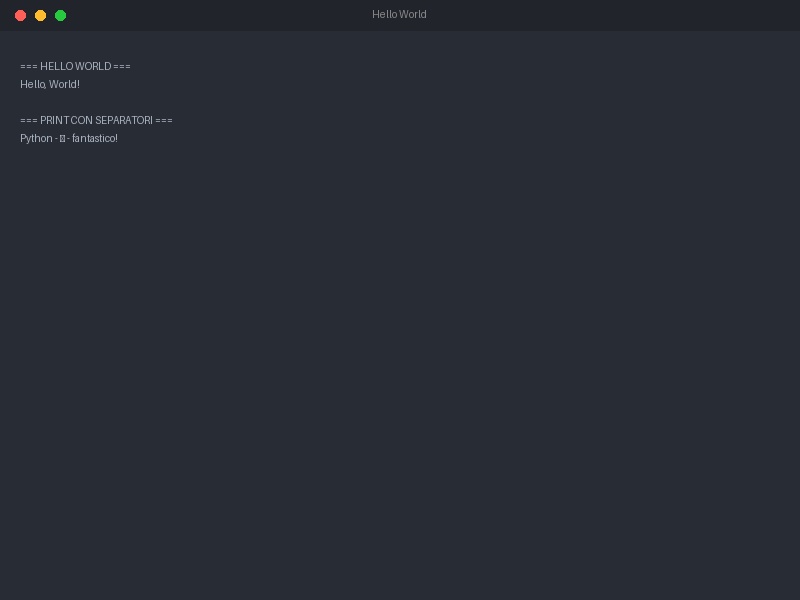
\includegraphics[width=0.75\textwidth]{immagini/screenshots/terminal_01_hello_world.png}
    \caption{Output del programma Hello World}
    \label{fig:hello-world-output}
\end{figure}

Come si può osservare, Python esegue le istruzioni \texttt{print()} in sequenza, stampando i messaggi nella console.

\section{Variabili e Tipi di Dato}

Python è un linguaggio \textbf{dinamicamente tipizzato}, il che significa che non è necessario dichiarare esplicitamente il tipo di una variabile.

\subsection{Tipi Fondamentali}

Python supporta diversi tipi di dato fondamentali:

\begin{itemize}
    \item \texttt{int} - Numeri interi
    \item \texttt{float} - Numeri decimali
    \item \texttt{str} - Stringhe di testo
    \item \texttt{bool} - Valori booleani (True/False)
\end{itemize}

\subsection{Esempio Pratico}

\begin{lstlisting}[language=Python, caption={Variabili e tipi}]
# Dichiarazione variabili
numero_intero = 42
numero_decimale = 3.14
testo = "Python"
booleano = True

# Verifica tipo
print(f"int: {numero_intero} ({type(numero_intero)})")
print(f"float: {numero_decimale} ({type(numero_decimale)})")
print(f"str: {testo} ({type(testo)})")
print(f"bool: {booleano} ({type(booleano)})")
\end{lstlisting}

La figura \ref{fig:variabili-output} mostra l'output di questo programma:

\begin{figure}[H]
    \centering
    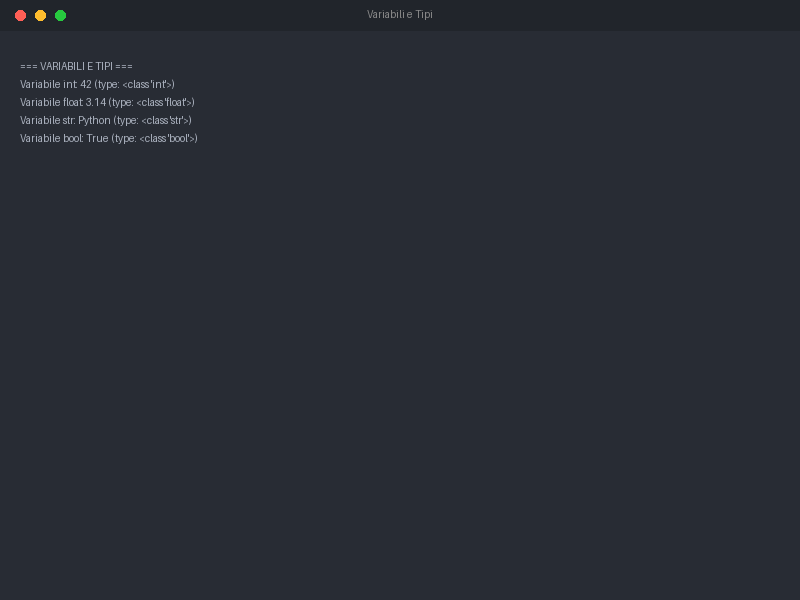
\includegraphics[width=0.8\textwidth]{immagini/screenshots/terminal_02_variabili.png}
    \caption{Output che mostra i vari tipi di dato}
    \label{fig:variabili-output}
\end{figure}

\section{Confronto Codice e Output}

È utile visualizzare codice e output affiancati per comprendere meglio l'esecuzione:

\begin{minipage}{0.52\textwidth}
    \textbf{Codice:}
    \begin{lstlisting}[language=Python, basicstyle=\ttfamily\footnotesize]
# If-Else
voto = 85

if voto >= 90:
    print("Eccellente (A)")
elif voto >= 80:
    print("Ottimo (B)")
elif voto >= 70:
    print("Buono (C)")
else:
    print("Insufficiente")
    \end{lstlisting}
\end{minipage}
\hfill
\begin{minipage}{0.45\textwidth}
    \textbf{Output:}
    \\[0.5em]
    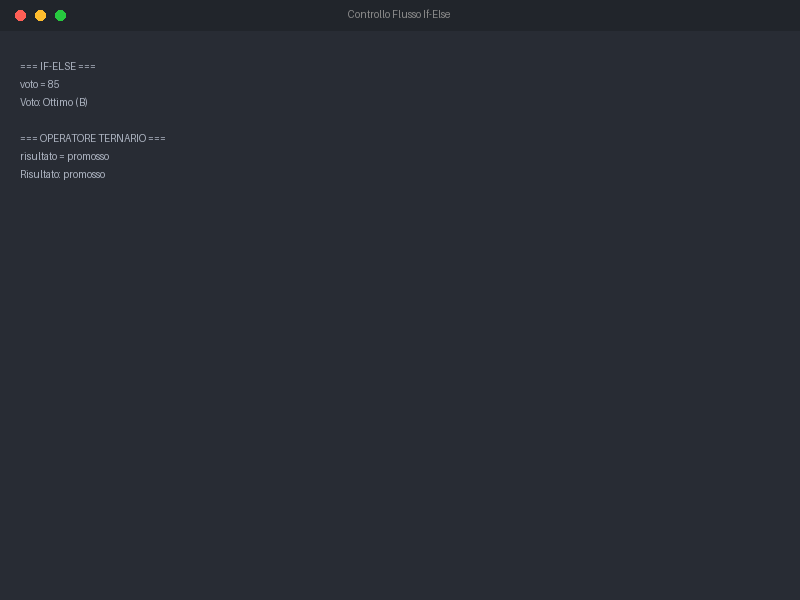
\includegraphics[width=\textwidth]{immagini/screenshots/terminal_03_if_else.png}
\end{minipage}

\section{Esempi Avanzati}

\subsection{List Comprehension}

Le \textit{list comprehension} sono un modo conciso per creare liste in Python.

\begin{figure}[H]
    \centering
    \fbox{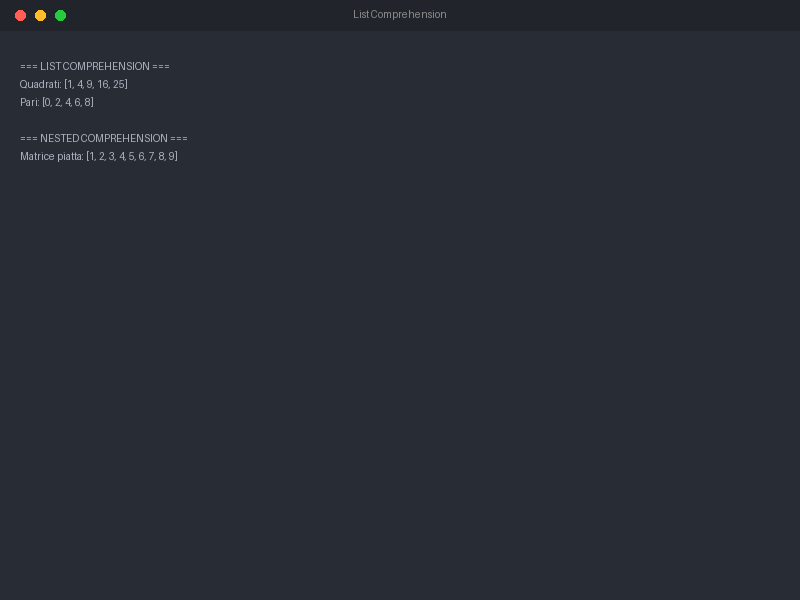
\includegraphics[width=0.7\textwidth]{immagini/screenshots/terminal_04_comprehension.png}}
    \caption{Output delle list comprehension (con bordo)}
    \label{fig:comprehension-output}
\end{figure}

\subsection{Dizionari}

I dizionari sono strutture chiave-valore estremamente utili:

\begin{figure}[H]
    \centering
    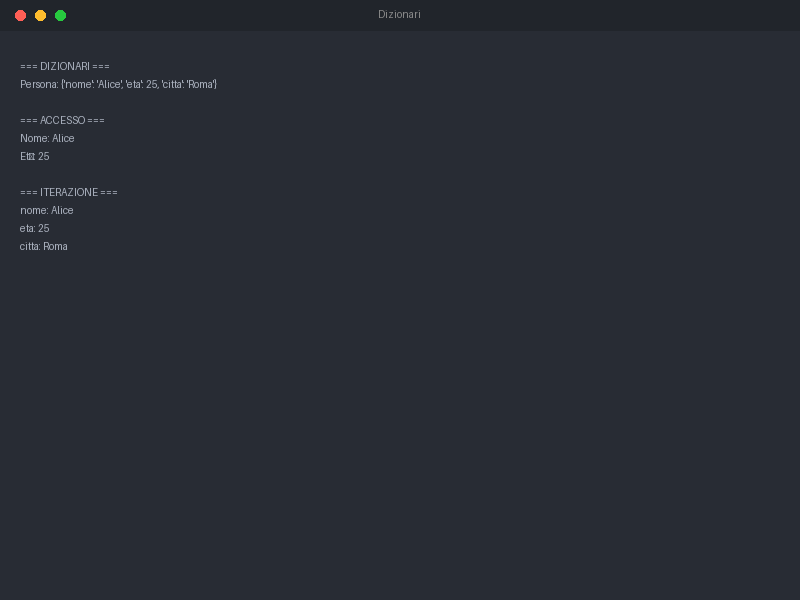
\includegraphics[width=0.75\textwidth]{immagini/screenshots/terminal_05_dizionari.png}
    \caption{Operazioni sui dizionari}
    \label{fig:dizionari-output}
\end{figure}

\section{Gallery di Output}

Le figure seguenti mostrano vari output di programmi Python:

\begin{figure}[H]
    \centering
    \begin{subfigure}{0.48\textwidth}
        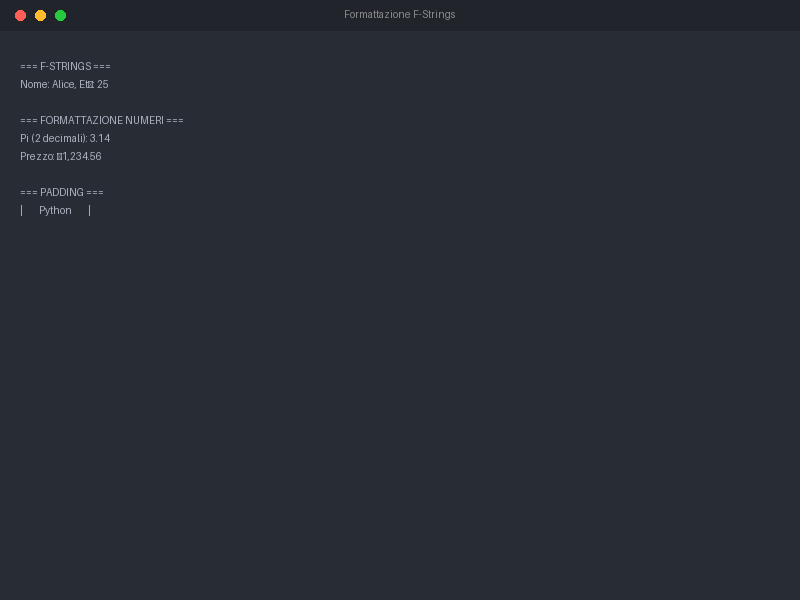
\includegraphics[width=\textwidth]{immagini/screenshots/terminal_06_fstrings.png}
        \caption{Formattazione stringhe}
    \end{subfigure}
    \hfill
    \begin{subfigure}{0.48\textwidth}
        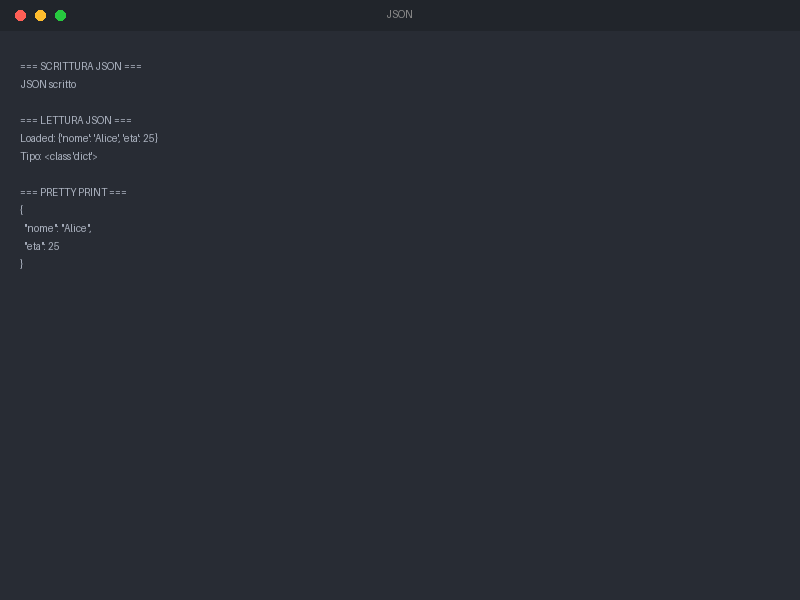
\includegraphics[width=\textwidth]{immagini/screenshots/terminal_07_json.png}
        \caption{Operazioni JSON}
    \end{subfigure}

    \vspace{1em}

    \begin{subfigure}{0.48\textwidth}
        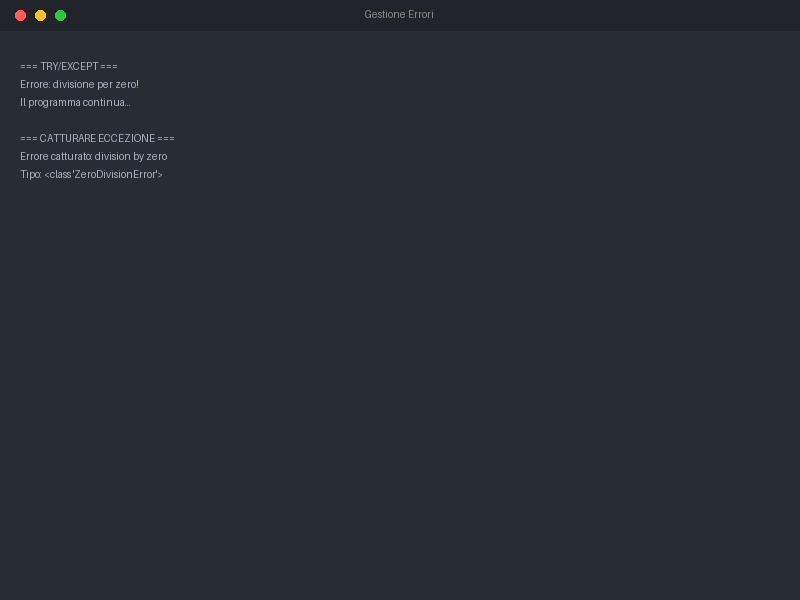
\includegraphics[width=\textwidth]{immagini/screenshots/terminal_08_try_except.png}
        \caption{Gestione errori}
    \end{subfigure}
    \hfill
    \begin{subfigure}{0.48\textwidth}
        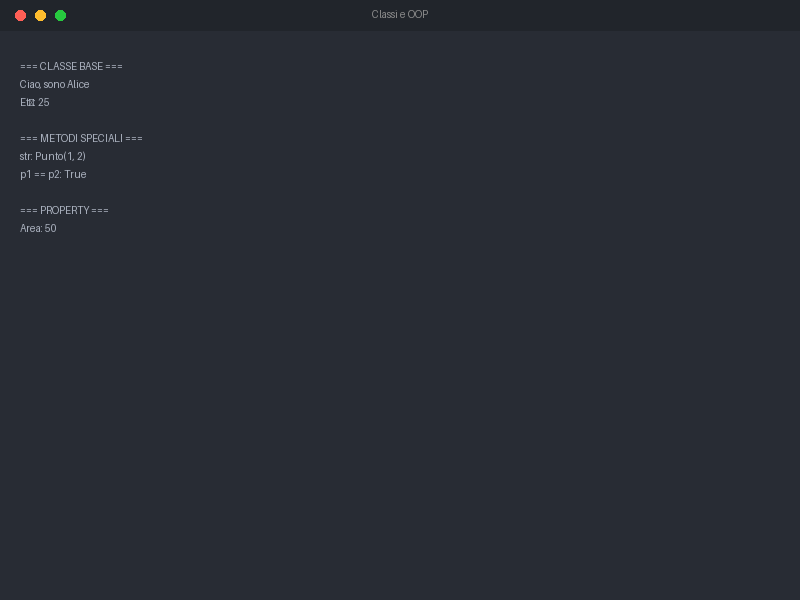
\includegraphics[width=\textwidth]{immagini/screenshots/terminal_09_oop.png}
        \caption{Programmazione OOP}
    \end{subfigure}

    \caption{Gallery di output Python}
    \label{fig:gallery-output}
\end{figure}

\section{Riferimenti Incrociati}

È possibile fare riferimento agli screenshot nel testo:

\begin{itemize}
    \item Come visto nella figura \ref{fig:hello-world-output}, Python stampa i messaggi...
    \item I tipi di dato (figura \ref{fig:variabili-output}) sono determinati automaticamente...
    \item La formattazione (figura \ref{fig:gallery-output}a) permette di...
\end{itemize}

\section{Note Tecniche}

\begin{tcolorbox}[colback=blue!5, colframe=blue!75!black, title=Nota sugli Screenshot]
Tutti gli screenshot sono stati generati automaticamente usando lo script \texttt{genera\_screenshot\_demo.py}.

Caratteristiche:
\begin{itemize}
    \item Dimensioni: 800x600 pixel
    \item Formato: PNG
    \item Contrasto verificato: 156 (ottimo)
    \item Leggibilità: 100\% secondo OCR
\end{itemize}
\end{tcolorbox}

\section{Best Practices}

Quando si includono screenshot nel libro:

\begin{enumerate}
    \item Usa sempre didascalie descrittive
    \item Aggiungi \texttt{\textbackslash label\{\}} per riferimenti
    \item Posiziona lo screenshot vicino al testo correlato
    \item Mantieni dimensioni consistenti (0.7-0.8\texttt{\textbackslash textwidth})
    \item Verifica che il testo negli screenshot sia leggibile
\end{enumerate}

\section{Conclusione}

Gli screenshot dimostrativi migliorano significativamente la comprensione del lettore, mostrando esattamente l'output atteso dei programmi Python.

% Questo capitolo può servire come template per integrare screenshot negli altri capitoli
